\section{Measurements of $\phi_s$ and $\Delta\Gamma_s$}
\label{sec:phisdgs}

The $\phi_s$ weak phase and $B_s$ meson decay width difference can
be extracted by a time dependent full angular decay analysis of the 
$B^0_s \to J/\psi \phi$ decays.

The results that the ATLAS and CMS Experiments obtained on their Run1
datasets are:
\begin{eqnarray}
  \phi_s & = & -0.090 \pm 0.078 (\mbox{stat}) \pm 0.041 (\mbox{syst})\:[\mbox{rad}] \\
  \Delta\Gamma_s & = & \phantom{-}0.085 \pm 0.011 (\mbox{stat}) \pm 0.007 (\mbox{syst})\:[\mbox{ps}^{-1}]
\end{eqnarray}
for ATLAS \cite{atlas_phis_8TeV} and:
\begin{eqnarray}
  \phi_s & = & -0.075 \pm 0.097 (\mbox{stat}) \pm 0.031 (\mbox{syst})\:[\mbox{rad}] \\
  \Delta\Gamma_s & = & \phantom{-}0.095 \pm 0.013 (\mbox{stat}) \pm 0.007 (\mbox{syst})\:[\mbox{ps}^{-1}]
\end{eqnarray}
for CMS \cite{cms_phis}. As can be seen in Fig.~\ref{phis_atlas_cms} both measurements are in
excellent agreement with the SM expectations.

\begin{figure}
  \begin{center}
    \begin{tabular}{c c}
      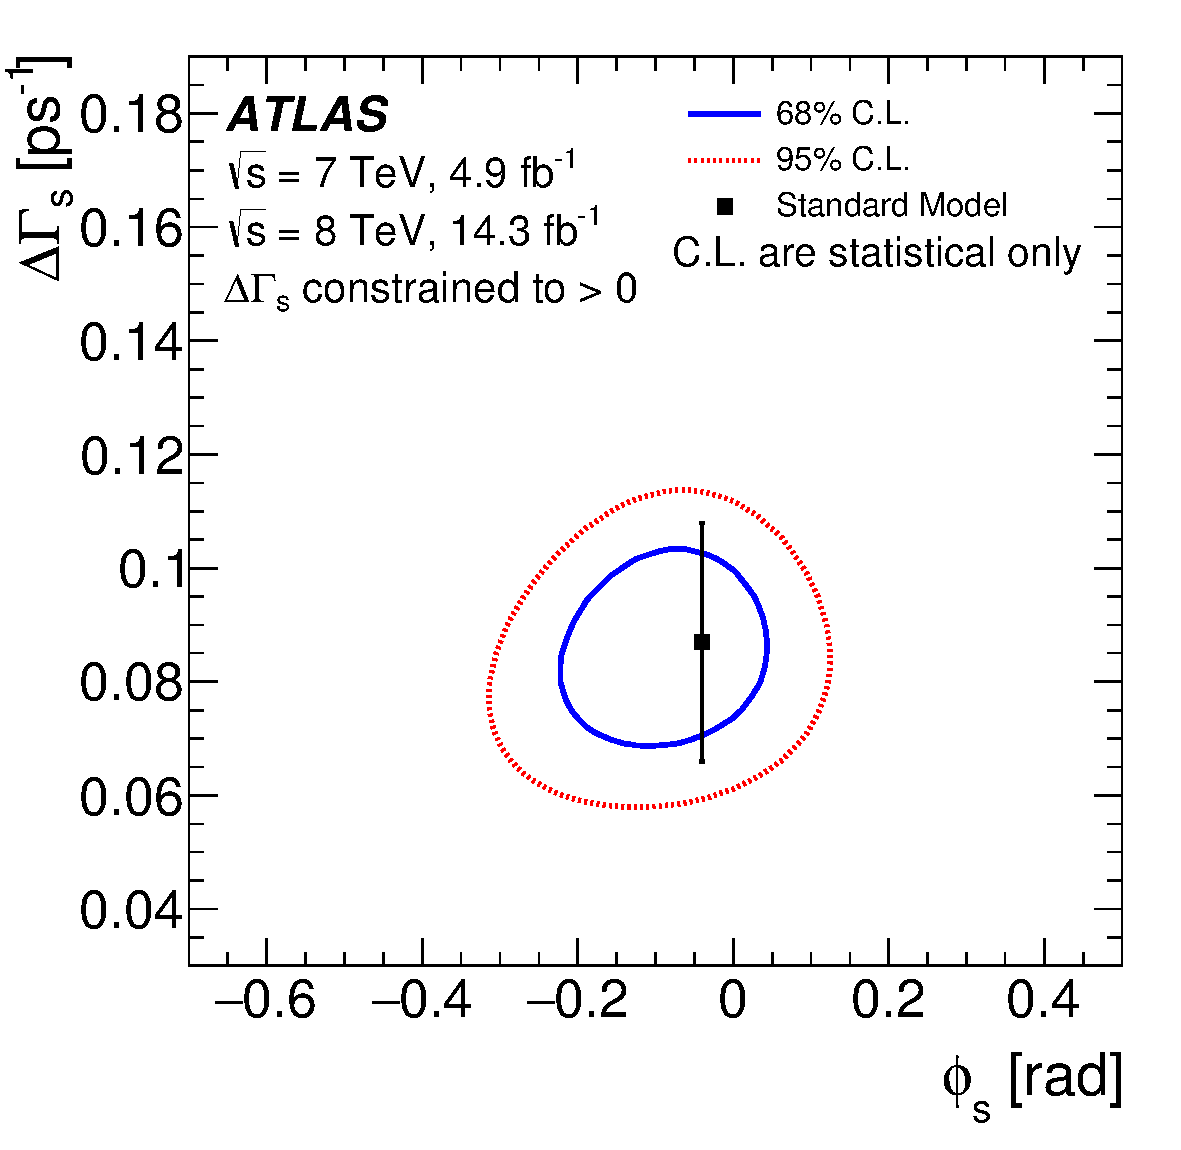
\includegraphics[height=5cm]{figs/atlas_phis_result.pdf} &
      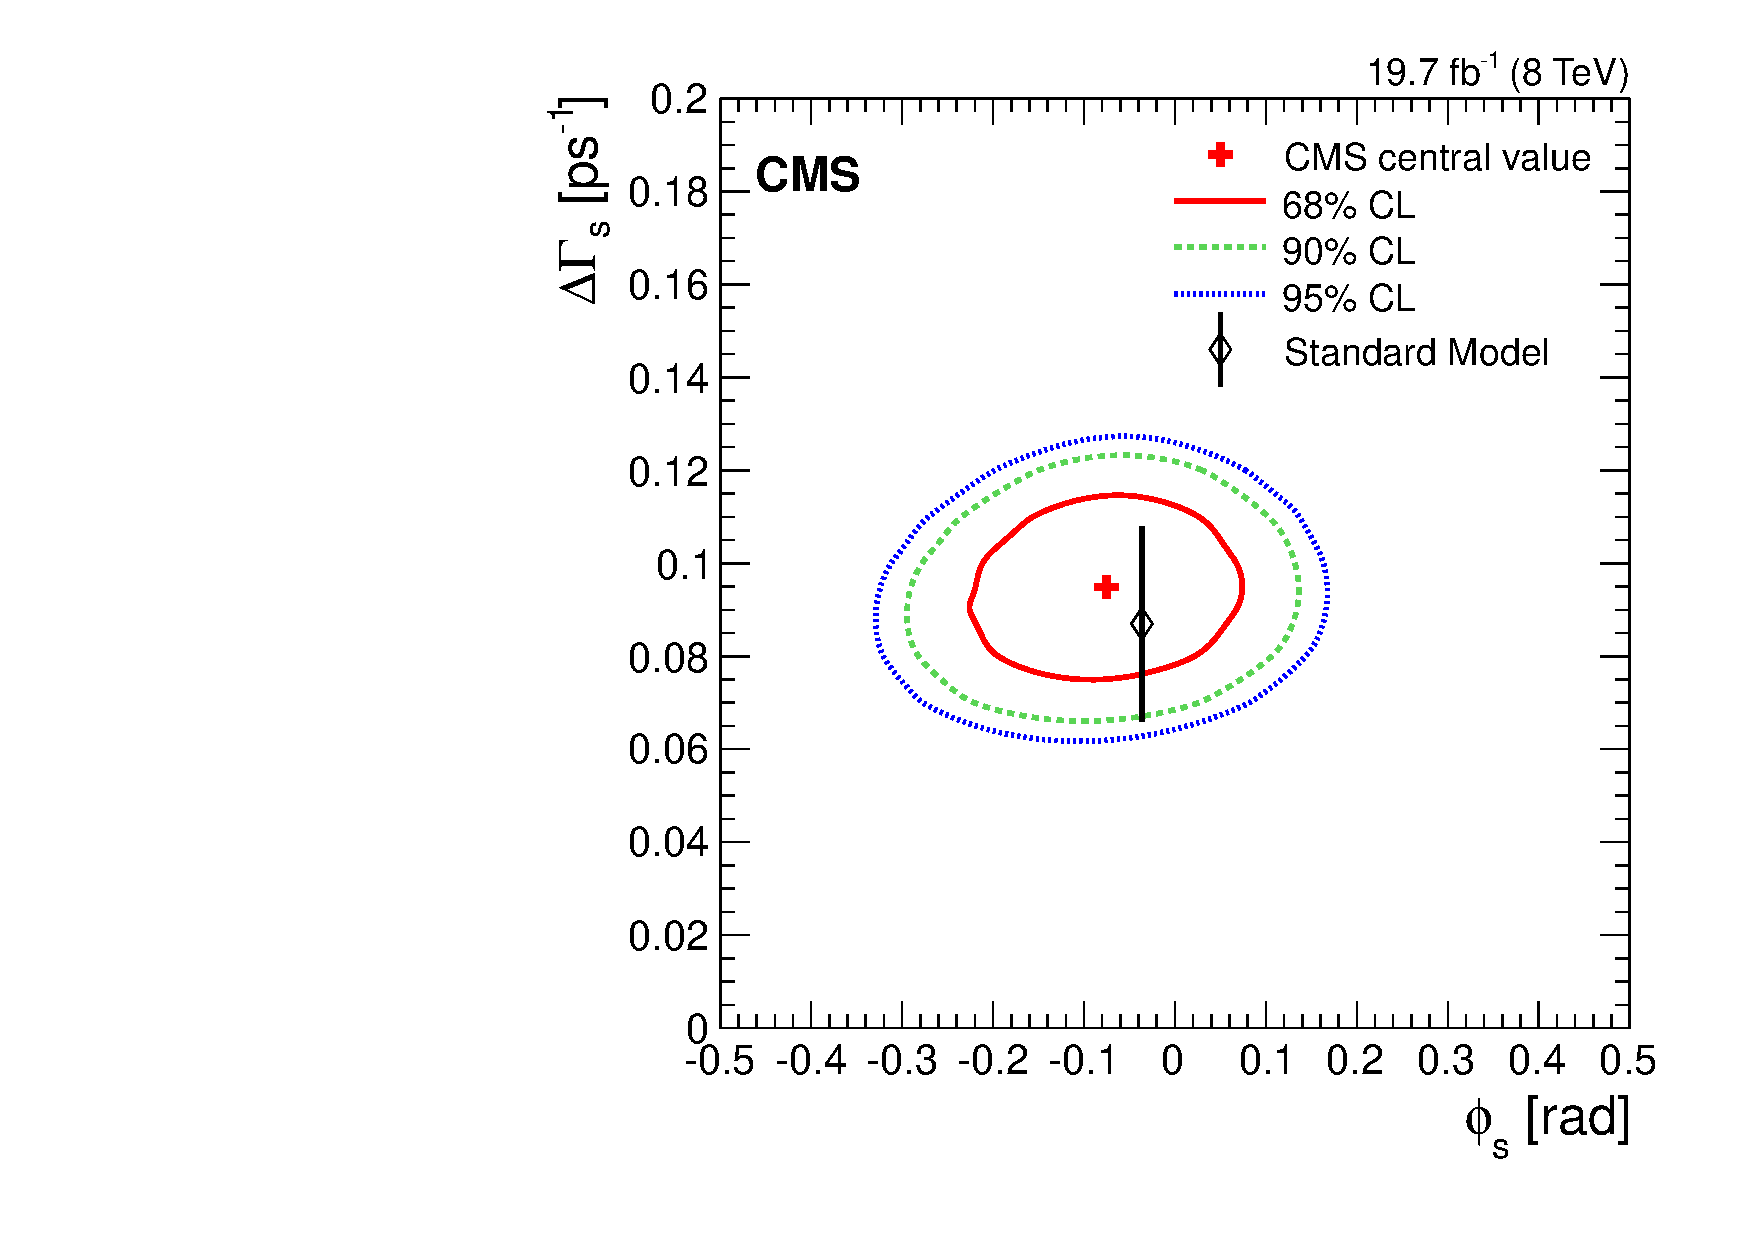
\includegraphics[height=5cm]{figs/cms_phis_result.pdf} 
    \end{tabular}
  \end{center}
  \caption{\label{phis_atlas_cms}Results on $\phi_s$ and $\Delta\Gamma_s$ from
  $B^0_s \to J/\psi \phi$ decays from ATLAS (left figure) and CMS.}
\end{figure}
